\documentclass{article}
\usepackage{pgf}
\usepackage{pgfpages}

\usepackage{amsmath}
\pgfpagesdeclarelayout{boxed}
{
  \edef\pgfpageoptionborder{0pt}
}
{
  \pgfpagesphysicalpageoptions
  {%
    logical pages=1,%
  }
  \pgfpageslogicalpageoptions{1}
  {
    border code=\pgfsetlinewidth{2pt}\pgfstroke,%
    border shrink=\pgfpageoptionborder,%
    resized width=.95\pgfphysicalwidth,%
    resized height=.95\pgfphysicalheight,%
    center=\pgfpoint{.5\pgfphysicalwidth}{.5\pgfphysicalheight}%
  }%
}

\pgfpagesuselayout{boxed}
\usepackage[utf8]{inputenc}
\usepackage{graphicx}
\usepackage{fancyhdr}
\usepackage{xcolor}
\usepackage{calrsfs}
\newtheorem{definition}{Definition}[section]
\DeclareMathAlphabet{\pazocal}{OMS}{zplm}{m}{n}
\newcommand{\Lb}{\pazocal{L}}
\newcommand{\Mb}{\mathcal{M}}
\newcommand{\Bb}{\mathcal{B}}
\newcommand{\Rb}{\mathcal{R}}
\usepackage[backend=bibtex,natbib=true]{biblatex}
\addbibresource{References.bib}

\title{\textbf{High Order Essentially Non-Oscillatory Schemes and Weighted Essentially Non-Oscillatory Schemes for Selected Riemann Problems}}
\author{\textbf {Author: }\textbf{Abdul Rab}}
\date{\textbf \today}

\pagestyle{fancy}
\fancyhf{}
\lhead{\textcolor{gray}{High Order Weighted Essentially Non-Oscillatory Schemes}}
\begin{document}

\maketitle
\begin{center}
    \textbf{THESIS RESEARCH PROPOSAL \\A research thesis proposal submitted to the Department of\\ Mathematics and Social Science\\Sukkur IBA University, Sukkur\\ \medskip in partial fulfillment of the requirements for the degree of\\Master of Science in Mathematics\\ \medskip Thesis Supervisor: Dr. Sidrah Ahmed}
\end{center} 

\begin{figure}[h]
    \centering
    
\includegraphics[height = 2.5in]{IBA.jpg}
    \label{fig:my_label}
\end{figure}
\begin{center}
    \textbf {Department of Mathematics and Social Science}
\end{center}

\begin{center}
    \Huge{\textbf{Sukkur IBA University}}
\end{center}
\newpage

\tableofcontents

\section*{\textbf{Abstract}}
The proposed work is based on the formulation and applications of Essentially
non-oscillatory (ENO) and weighted ENO (WENO) schemes for solving
Riemann problems of hyperbolic equations with possibly discontinuous
solutions or solutions with sharp gradient regions. The construction process of
ENO and WENO schemes \cite{shu_2020} involves an approximation procedure, in such a way
that the high order accuracy is achieved in smooth regions and the shocks or
other discontinuous sharp gradients are obtained as essentially nonoscillatory solutions, hence these schemes are especially suitable for the
problems containing both strong discontinuities and complex smooth solution
features. In this work, I will present the basic formulation of WENO schemes
and sample applications from computational fluid dynamics and traffic flow
problems. Finally, an extension to the currently applied WENO schemes will
be mentioned.


\paragraph{\textbf{Key Words:}}
Numerical Solutions to Partial Differential Equations; Essentially Non-Oscillatory Method (ENO); Weighted ENO (WENO); Finite Voume Method (FVM);

\section{Introduction}
 The need of numerical solution to partial differential equation arises when analytical solution is difficult to find or it's closed form almost surely does not exist. This difficulty become more evident while solving non-linear partial differential equations. The problem get worse when the system of partial differential eqations are equipped with discontinuous initial data profile. As in this case we can no longer establish a solution to the system of PDEs in strong or classical sense. A class of such systems are classified as hyperbolic conservation laws. This classification is based on special structure of the eigenvalues of jacobian matrices related to the flux vector of conservation law. The complex interaction of waves emerging in different regions between characteristics curves poses a major challenge to find the exact as well as numerical solution to hyperbolic conservation laws. In this struggle, it has been found that the consistent and stable numerical solution to hyperbolic conservation laws are also difficult to achieve. Several methods have been formulated for finding the numerical solution to nonlinear conservation laws. These methods include high order accurate schemes such as Finite Volume Method (FVM), Finite difference method (FDM), Finite Element Method (FEM), and Spectral schemes. The primary concern is to find a smooth and regulator solution which requires a higher order accuracy as well as computational efficiency of the method. The first order accurate schemes gives the solution to hyperbolic PDEs, but to get the desired accuracy mesh size should be kept very close to zero. which in turn makes computation cost very high and slows the overall clock speed. Hence it is essential to formulate a procedure that is more accurate and involves less computations.  
In fact, by the famous Godunov theorem, a linear scheme must be either oscillatory or only first order accurate. So, in this regard the new scheme, Essentially Non-Oscillatory (ENO) Scheme, proposed in (\cite{harten1987uniformly})  approximates the solution with high order accuracy in smooth regions and helps us smooth transitions of essentially non-oscillatory discontinuities.


\section{Definitions}
% \noindent \textbf{Brief introduction to Hyperbolic Conservation Laws}\\
% Here you have to give definition of hyperbolic conservation laws, Riemann problem, the characteristics curve and some discussion on solution of hyperbolic conservation laws. \\
% 
\noindent \textbf{Hyperbolic conservation law} \\
A conservation law states that a particular measurable property of an isolated physical system does not change as the system evolves over time. Exact conservation laws include conservation of mass, conservation of linear momentum, conservation of angular momentum, and conservation of electric charge. Hyperbolic PDEs of the following form happens to satisfy the conservation law.
\begin{equation}
    \frac{\partial }{\partial t}u(x,t) + \frac{\partial }{\partial x}f(u(x,t)) = 0
\end{equation}
Here $u(x,t)$ represents the quantity that moves according to the given flux function $f(u(x,t))$.\\

\noindent \textbf{Riemann Problem} \\
A Riemann problem, named after Bernhard Riemann, is a specific initial value problem composed of a conservation equation together with piece-wise constant initial data which has a single discontinuity in the domain of interest.\\

\noindent \textbf{Characteristic Curves}\\
The method of characteristics discovers curves (called characteristic curves or just characteristics) along which the PDE becomes an ordinary differential equation (ODE). Once the ODE is found, it can be solved along the characteristic curves and transformed into a solution for the original PDE.\\

\noindent \textbf{Conservative Numerical Method}\\
A numerical method is conservative if it can be written in the following form 
\begin{equation}
    U^{n+1}_{j} = U^n_j - \frac{k}{h} \left[ F(U^n_{j-p},\cdots,U^n_{j+q} ) - F(U^n_{j-p-1},\cdots,U^n_{j+q-1} )  \right]
\end{equation}
where $F$ has $p+q+1$ arguments.\\

\noindent \textbf{Consistent Numerical Method}\\
A conservative method is consistent with original consservation law if $F(u)$ reduces to $f(u)$ i.e. $F(\bar{u,\cdots,\bar{u}}) = f(\bar{u})$\\

\noindent \textbf{Convergent Scheme}\\
A consistent and conservative method converges to a weak solution everywhere as $k,h \longrightarrow 0$ and $\frac{k}{h}$ satisfies stability conditions.\\

\noindent \textbf{Linear Scheme}\\
A linear scheme is one that can be written in the form
\begin{equation}
\bar{u}_{j}^{n+1} = \sum_{\ell=-k}^{k} c_{\ell}(\lambda) \bar{u}_{j+\ell}^{n}, \;\;\;\lambda = \frac{\Delta t}{\Delta x}    
\end{equation}
\noindent when applied to a linear conservation law.\\

\noindent \textbf{Monotone Schemes}\\
A monotone scheme is one that can be written in the form
\begin{equation}
  \bar{u}_{j}^{n+1} = \mathcal{H}(\bar{u}_{j-p}^{n}, \dots, \bar{u}_{j+q}^{n}),
\end{equation}
\noindent where $\mathcal{H}$ is a non decreasing function in all arguments.\\

\noindent \textbf{Total Variation Diminishing Scheme}\\
A total variation diminishing scheme is one that can be written in the form
\begin{equation}
    TV(U^{n+1}) \leq TV(U^{n})
\end{equation}
\noindent where
\begin{equation}
    TV(U) = \sum |U_{j+1} - U_j|
\end{equation}
\\

\section{Problem Statement}
\noindent The problem is taken from the article A solution of the Junction Riemann Problem for 1D hyperbolic balance laws in networks including supersonic flow conditions on elastic collapsible tubes. Which is a mathematical model in the form of hyperblic PDE i.e. holds convservation law. Our task is to apply ENO and WENO Finite Volume scheme on this model to get the desired results. Moreover I will examine the above listed properties of ENO and WENO procedures for the proposed model in the given article\cite{murillo2021solution}. 

\section{Literature Review}
ENO and WENO scheme has been discussed in detail ~(\cite{shu_2020}). and Model that has been proposed in problem statement section will be solved numerically using Finite Volume Method with the aid of Nonlinear ENO/WENO scheme.


\section{Methodology}
The essentially non-oscillatory (ENO) scheme is an ENO approximation procedure, consists of two parts i.e. ENO interpolation procedure  and ENO reconstruction procedure. So we go through them one by one. In ENO scheme, the interpolation is done to approximate higher order cell averages of unknown $u$. Let's demonstrate the interpolation in one dimensional case. Assume that $u(x)$ is piece wise continuous solution to given hyperbolic conservation law i.e.
\begin{align}
u_{t} + f(u)_{x} = 0  &\text{ in } \mathbb{R} \times [0,\infty)\\ 
u(x,0) = u_{0}(x) &\text{ on } \mathbb{R} \times \{t=0\}
\end{align}

\noindent In numerical approximations, the first step is to generate the computational domain. In case of one dimension, given the real line as $a\leq x \leq b$ then the  mesh $x_1<x_2<x_3<...<x_n$ with $\Delta x_{i+\frac{1}{2}} = x_{i+1} - x_i$ and $\Delta x = \max_i{\Delta x_{i+\frac{1}{2}}}$

\noindent Let $u_i = u(x_i)$ be discrete set of values of $u(x)$. we want to find an interpolating polynomial $P_{i+\frac{1}{2}}(x)$ on $I_{i+\frac{1}{2}} = (x_i,x_{i+1})$ for u(x). This can be done with the help of classical interpolation method as Newton Method or Lagrange Method. 


\noindent Suppose we have four points central stencil i.e. $S = \{x_{i-1},x_i,x_{i+1},x_{i+2}\}$ using this we get an unique high order polynomial $P_{i+\frac{1}{2}}(x)$ of degree 3 with following conditions satisfied.
\begin{equation}
    P_{i+\frac{1}{2}}(x_j) = u_j \hspace{2cm} j=i-1,i,i+1,i+2
\end{equation}
\noindent The solution is smooth in the chosen stencil if the following condition is met
\begin{equation} \label{HighOrderCondition}
    |u(x) - P_{i + \frac{1}{2}}(x)| \leq C \Delta x ^4, \hspace{2cm} x \in I_{i + \frac{1}{2}}
\end{equation}

\noindent The actual problem is to get smoothness of solution and it's gradient near discontinuities. The solution breaks to be high order accurate if chosen stencil contains the discontinuity i.e. it fails the condition (\ref{HighOrderCondition}).

\noindent The idea of ENO \cite{harten1987uniformly} is to pick the stencil in such a way that local smoothness of solution $u(x)$ is guaranteed. In order to choose stencil adaptively and automatically, Newton divided difference is used

\begin{enumerate}
    \item Compute $u(x)$ using divided difference, for all $j= ...1,2,3...$
    \begin{equation}
        u[j,0] = u_j,
    \end{equation}
    then for $k = 0,1,...$ and all $j$,
    \begin{equation}
        u[j,k+1] = \frac{u[j+1,k] - u[j,k]}{x_{j+k+1} - x_j}
    \end{equation}
    \item Initial must contain only two points of the chosen interval $I_{i+\frac{1}{2}}$
    \begin{equation}
        S^{( 0 )} = \{ x_i,x_{i+1} \}
    \end{equation}
\end{enumerate}
\noindent at each iteration the only one point is added to keep intact the smoothness.\\

\noindent \textbf{ENO reconstruction} procedure is followed to tackle the hyperbolic PDEs i.e. Conservation Laws. Now we use different notation which is widely used in \textbf{Finite Volume Scheme}.
\begin{align}
    &\text{Control Volume or Cell } I_i = (x_{i - \frac{1}{2}},x_{i + \frac{1}{2}})\\
    &\text{Cell Size } \Delta x = x_{i + \frac{1}{2}} - x_{i - \frac{1}{2}}\\
    &  \Delta x =\max_i \Delta x_i
\end{align}
Cell averages are assumed to be given initially
\begin{equation}
     \bar{u}_{i} = \frac{1}{\Delta x_i} \int_{x_{i - \frac{1}{2}}}^{x_{i + \frac{1}{2}}} u(x)\;dx , \;\;\;i \in \{\dots1,2,3,\cdots\}.
\end{equation}

\noindent the task is to find high order polynomial $p_i(x)$ with high order accuracy whenever $u(x)$ is in smooth region. As discussed previously in the interpolation procedure, the reconstruction procedure follows the similar strategy. The reconstruction procedures takes the stencil e.g. a central stencil $S = \{ I_{i-1},I_i, I_{i+1}\}$, and find the quadratic polynomial $p_i(x)$ such that it satisfies the following condition.
\begin{equation}
     \bar{u}_{j} = \frac{1}{\Delta x_j} \int_{x_{j - \frac{1}{2}}}^{x_{j + \frac{1}{2}}} p_i(x)\;dx , \;\;\; j=i-1,i,i+1
\end{equation}

\noindent existence and uniqueness of reconstruction polynomials $p_i(x)$ can be proved but here preferred procedure will be to reconstruct $p_i(x)$ it via primitive functions. and then apply ENO procedure.

\begin{equation}
    U(x) = \int _a^x u(\xi) d\xi 
\end{equation}

\noindent here $a= x_{i0 - \frac{1}{2}} $ and first cell to compute is $I_{i0}$. we get $U(x_{io - \frac{1}{2}}) = 0$ and for all $i \leq i_0$,
\begin{equation}
    U(x_{i+\frac{1}{2}}) = \int_{x_{i0 - \frac{1}{2}}}^ {x_{i + \frac{1}{2}}} u(\xi) d\xi = \sum_{j=i_0}^{i} \int_{x_{j - \frac{1}{2}}}^ {x_{j + \frac{1}{2}}} u(\xi) d\xi = \sum_{j=i_0}^{i} \bar{u_j} \Delta x_j.
\end{equation}

\noindent having cell averages $\bar{u_j}$ of $u(x)$, then we have face values i.e. $U(x_{i + \frac{1}{2}})$ of the primitive function $U(x)$. ENO interpolation procedure can implemented for $U(x)$ to find cubic interpolation polynomial $P_i(x)$ by using central stencil i.e. $\Tilde{S} = \{ x_{i-\frac{3}{2}},x_{i-\frac{1}{2}} , x_{i+\frac{1}{2}} , x_{i+\frac{3}{2}} \}$ satisfying

\begin{equation}
    P_i(x_{j+\frac{1}{2}}) = U(x_{j+\frac{1}{2}}) \;\;\; j = i-2,i-1,i,i+1
\end{equation}

\noindent and quadratic reconstruction polynomial $p_i(x)$ of $u(x)$ at central stencil  $S = \{ I_{i-1},I_i, I_{i+1}\}$ can be found as  $p_i(x) = \frac{d}{dx} P_i(x)$. Is can be shown that 

\begin{equation}
     \frac{1}{\Delta x_j} \int_{x_{j - \frac{1}{2}}}^{x_{j + \frac{1}{2}}} p_i(\xi)\;d\xi = \bar{u}_{j} , \;\;\; j=i-1,i,i+1
\end{equation}
\noindent it has been observed that whenever ENO reconstruction polynomial is needed we just take the derivative of ENO interpolation polynomial. There is no need to compute the divided differences of $U(x)$ because it can be written in term of $\bar{u_j}$ as show below.

\begin{equation}
    U[i-\frac{1}{2},1] = \bar{u_i}
\end{equation}

\noindent \textbf{One Dimensional Scalar equation} let's develop the ENO/WENO finite volume scheme for hyperbolic conservation law
\begin{equation}\label{conservation}
    u_t + f(u)_x = 0
\end{equation}

\noindent by integrating the conservation law (\ref{conservation}) over control volume or cell $I_i = (x_{i - \frac{1}{2}}, x_{i+ \frac{1}{2}} )$ then the integral form is
\begin{equation}
    \frac{d}{dt} \bar{u_i} + \frac{1}{\Delta x_i} \left(  f(u_{i+\frac{1}{2}}) -f(u_{i-\frac{1}{2}} ) \right)= 0
\end{equation}
\noindent where $\bar{u_i} = \frac{1}{\Delta x} \int_{x_{i - \frac{1}{2}}}^{x_{i + \frac{1}{2}}} u(x,t)dx $ is the spatial cell average of $u(x,t)$. To apply finite volume scheme the underlying variable is kept as cell averages i.e. $\{\bar{u_i} \}$ and ENO/WENO reconstruction procedures are used to approximate the face values i.e. $u_{i+\frac{1}{2}}$. To ensure stability, two reconstructed values $u^-_{i+\frac{1}{2}}$ and $u^+_{i + \frac{1}{2}}$ are computed in $I_i$ and $I_{i+1}$ respectively. By using both values in numerical flux function $\hat{f}$ we obtain the semi-discrete finite volume scheme as
\begin{equation}
    \frac{d}{dt} \bar{u_i} + \frac{1}{\Delta x_i} \left[ \hat{f}(u^{-}_{i+\frac{1}{2}},u^{+}_{{i+\frac{1}{2}}}) - \hat{f}(u^-_{i-\frac{1}{2}} , u^+_{i-\frac{1}{2}} ) \right] = 0
\end{equation}
\noindent We will choose the Godunov numerical flux. Further detailed introduction can be found in (LeVeque 1990). The ENO reconstruction procedure is used to approximate $u^-_{i+\frac{1}{2}}$ with starting cell $I_i$ in the stencil, then adding one cell at a time until required number of cells are reached. The ENO reconstruction procedure to approximate the $u^+_{i+\frac{1}{2}}$ at same location but starting with cell $I_{i+1}$ in the stencil.\\

The follwing is the Godunov numerical flux that will be used in ENO/WENO finite volume scheme.
\begin{equation}
\hat{f}(\bar{u}_{j}, \bar{u}_{j+1}) = 
\begin{cases}
\min_{\bar{u}_{j} \leq u \leq \bar{u}_{j+1}} f(u), &\bar{u}_{j} \leq  \bar{u}_{j+1}\\ 
\max_{\bar{u}_{j} \geq u \geq \bar{u}_{j+1}} f(u), &\bar{u}_{j} > \bar{u}_{j+1}.
\end{cases}
\end{equation}




\begin{figure}[h]
    \centering
    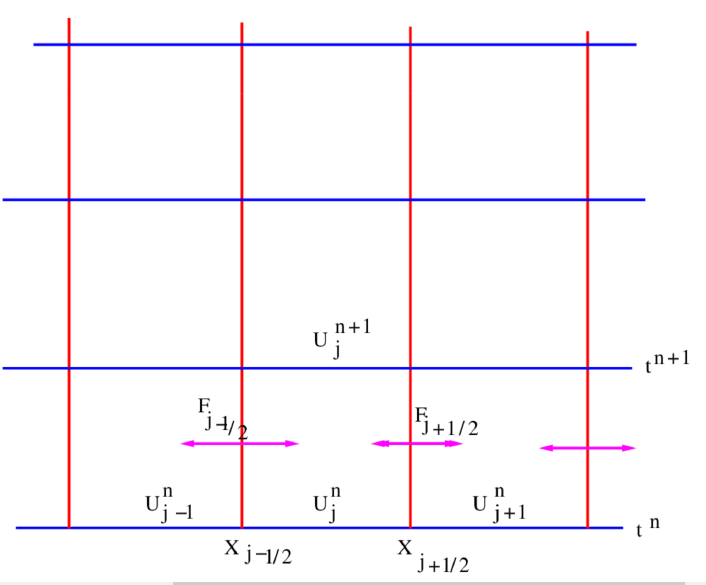
\includegraphics[width=12cm,height=10cm]{Screenshot 2022-01-23 212157.png}
    \caption{A typical finite volume grid displaying cell averages and fluxes.}
    \label{fig:my_label}
\end{figure}


\printbibliography
\end{document}